\documentclass[letterpaper, 12pt]{article}

\usepackage{blindtext}
\usepackage{graphicx}

\begin{document}

\newcommand{\textttEx}{\textbackslash{}texttt\{\}}
\newcommand{\textsfEx}{\textbackslash{}textsf\{\}}
\newcommand{\textrmEx}{\textbackslash{}textrm\{\}}

\newcommand{\rmfamilyEx}{\textbackslash{}rmfamily}
\newcommand{\sffamilyEx}{\textbackslash{}sffamily}
\newcommand{\ttfamilyEx}{\textbackslash{}ttfamily}

\newcommand{\emEx}{\textbackslash{}em}

%These commands allow changing the default font throughout the entire page
%the moment they are called
%\sffamily
%\rmfamily

\newcommand{\mylipsum}{}
\title{Example 4: Fonts}
\date{\today}
\author{Jave}
\maketitle

\section{\textsf{\LaTeX\ resources (\textsfEx) \textrm{on the internet (\textrmEx)} } }

The best place for downloaded LaTeX related software is CTAN\@.
Its address is \texttt{http://www.ctan.org} (\textttEx)\\


There are commands which require arguments, and then there are declarations which 
don't need arguments but affect any text that comes after.


If you don't want to specify where in the text you wish to change the font, declarations are needed
\begin{itemize}
  \item \rmfamily Roman font (\rmfamilyEx)
  \item \sffamily Sans-serif font (\sffamilyEx)
  \item \ttfamily Typewriter font (\ttfamilyEx)
\end{itemize}

If you do want to specify where in the text, arguments are needed. 
\begin{itemize}
  \item \textrm{Roman font} (\textrmEx)
  \item \textsf{Sans-serif font} (\textsfEx)
  \item \texttt{Typewriter font} (\textttEx)
\end{itemize}

\noindent To experiment the three pre-defined family fonts declarations.

  \subsection{The Roman font (default font with \rmfamilyEx)}
  \rmfamily  
  Lorem ipsum dolor sit amet, consectetur adipiscing elit, sed do eiusmod tempor incididunt ut labore et dolore magna aliqua. 

\ttfamily
  \subsection{\ttfamily The typewriter font (\ttfamilyEx)} 

  Lorem ipsum dolor sit amet, consectetur adipiscing elit, sed do eiusmod tempor incididunt ut labore et dolore magna aliqua. 

\sffamily 
  \subsection{The Sans-serif font (\sffamilyEx)} 
  \textbf{Notice that the subsection is not in sans-serif because (\sffamilyEx) is out of scope (outside the subsection command)}


  Lorem ipsum dolor sit amet, consectetur adipiscing elit, sed do eiusmod tempor incididunt ut labore et dolore magna aliqua. 

\rmfamily
\vspace{2.0mm}
These are some the commands and declarations that can be in Latex.


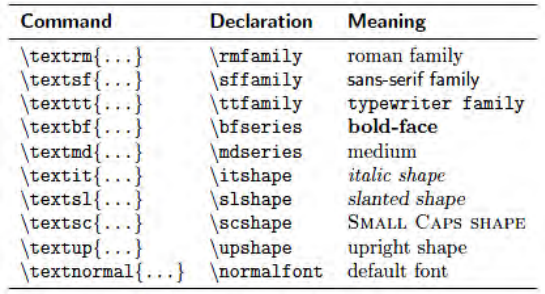
\includegraphics[width=\linewidth]{arguments_and_declarations.png}


But say, you want to use declarations but only for a long paragraph and not for the
entire document.
You use \{\} to basically help declarations identify the scope of the text that
follows it. For example,

\vspace{2.0mm}

In \LaTeX\@: \texttt{\{\sffamilyEx\ Whatever is inside the curly braces are in sans-serif\}}


Output: {\sffamily Whatever is inside the curly braces are in sans-serif}


\vspace{2.0mm}
\texttt{\{\emEx\ It can \{\emEx\ also\} be nested like this.\} Now I am out of the \emEx scope}


{\em It can{\em\ also} be nested like this.}\ Now I am out of the \emEx\ scope



\end{document}

 
